\documentclass[a4paper]{article}
\title{Realistic modelling of transmitter release at neocortical nerve terminals using CellBlender and MCell}
\author{Jaron Lee}
\usepackage{mathtools}
\usepackage{graphicx}
\usepackage{siunitx}
\usepackage{natbib}
\usepackage{hyperref}
\usepackage{tabularx}
\usepackage{enumerate}
\usepackage{extarrows}
\usepackage[hmargin=3cm,vmargin=3.5cm]{geometry}
\usepackage{amssymb}
\usepackage{amsmath}
\usepackage{float}
\setlength\parindent{0pt} % sets indent to zero
\setlength{\parskip}{10pt} % changes vertical space between paragraphs
\renewcommand\thesubsection{\thesection.\roman{subsection}}
\makeatletter
\renewcommand*\env@matrix[1][*\c@MaxMatrixCols c]{%
  \hskip -\arraycolsep
  \let\@ifnextchar\new@ifnextchar
  \array{#1}}
\makeatother
\DeclareSIUnit{\molar}{M}
\begin{document}
\maketitle

\section{Introduction}
This paper implements and investigates calcium buffering in a realistic model of a neocortical terminal. This implementation is achieved by utilisng CellBlender which has the MCell backend (see below).  A realistic model is created \textit{in silico} with the aim to simulate transmitter release from synaptic vesicles. We present our results in animated form. 

This project is motivated primarily by the importance of modelling in biology. Biological modelling can motivate scientific experiments by suggesting potential hypotheses for a particular phenomenon. Modelling can also assist in interpreting experimental results, by attempting to replicate a phenomenon by adjusting parameters in the model that are not observable in reality. A successful experiment can be subsequently supported by checking the proposed hypothesis in modelling software. Other uses of modelling involve the ability to produce high-quality diagrams and animations, which are useful for effectively communicating results both in papers and in presentations. A secondary aim of this project is to address the difficulty of accessing modelling technologies. It is uncommon for biologists to possess the requisite skills for modelling (though this is changing).
This project aims to fill this niche by providing a reproducible guide for the replication of the results obtained in this project, thus serving as an introduction to realistic modelling in neuroscience.

All the software utilised in this project are available to the public for free. Blender (ver. 2.71) is a 3D graphics modelling software which is free and traditionally used for applications such as digital media, games and the visual arts. MCell (ver. 3.2.1) is a cell simulation environment which provides a command-line interface to run Monte Carlo simulations to solve the diffusion equations at the molecular level (see \cite{stiles1996miniature}, \cite{stiles2001monte} and \cite{Kerr:SiamJSciComput:2008}). CellBlender (ver. 1.0 RC3) is a Blender add-on which allows the user to access the features of MCell through a Blender interface. Together with the general purpose language Python (ver. 3.4.2), this paper utilises these technologies to produce a step-by-step guide for simulating the calcium buffering and handling at neocortical nerve terminals.

The advantages of this CellBlender/MCell workflow in running such simulations are many-fold. Firstly, the user does not need to be familiar with programming through a command line interface to do cellular level modelling, enabling a wider audience to access the utility of a simulation environment. Secondly, the simulation results are presented in a Blender environment, allowing the user to manipulate and interact with the model to obtain a better interpretation of the model output. Thirdly, once the simulation has been set up, it is an easy task for the user to modify the model parameters and geometric configurations to explore their impact on the model results. 

All documentation, simulation files, scripts, tutorial instructions and this report can be found at \url{https://github.com/kanilor/cellblender_project}.

\section{Background Information}

\subsection{Synaptic Structure}
In this paper we consider the neocortical synapses of the layer V pyramidal cell type. These are excitatory synapses, which mean that action potentials invading the presynaptic neuron increase the probability of an action potential propagating through the postsynaptic cell. The synapse consists of the presynaptic terminal (the bouton) and the postsynaptic terminal (the spine). 

Axons of neighbouring neurons are interspersed with small swellings along their length, and at the terminal end of the axon. These swellings are termed boutons-en-passant (boutons for short), and at these locations transmitter release may occur. The bouton contain hundreds of synaptic vesicles and the associated infrastructure for vesicle release such as mitochondria, endoplasic reticulum, the presynaptic grid, the calcium and potassiums channels, autoreceptors, vesicular glutamate transporters, excitatory amino acid transporters, and the proteinacious release apparatus.

Dendrites of excitatory neurons are covered with spines, which are small protrusions consisting of a bulbous head and a thin neck, as per \cite{Arellano:FrontNeurosci:2007}. Their primary role is to compartmentalise individual synaptic inputs.

\subsection{Synaptic Transmission - An Overview}
An action potential propagates along the membrane of the presynaptic cell until it invades the synapse. This depolarisation causes voltage-gated calcium channels to open. Calcium ions flow from the extracellular space into the presynaptic terminal due to the concentration gradient. The entered calcium ions activate proteins (SNARE complex) in the nerve terminal, causing vesicle fusion with the synaptic cell membrane and emptying the contents of the vesicle (about 4700 molecules) into the synaptic cleft. The neurotransmitter molecules (glutamate) bind to AMPA or NMDA receptors on the postsynaptic density. At least two neurotransmitter molecules must bind to the receptor in order for activation. Activation of a postsynaptic glutamate receptor causes an influx of ions, predominantly sodium at resting membrane potential. The influx of ions will cause a depolarisation of the dendrite at the postsynaptic terminal, which produces a postsynaptic potential. Neurotransmitter molecules which are not bound to postsynaptic receptors diffuse into the extracellular space and are taken up predominantly by glial cells (astrocytes). 


\subsection{Vesicles}
At each synapse, there are hundreds of vesicles putatively filled with neurotransmitters. In the case of excitatory synapses, the transmitter is typically glutamate. Each vesicle is filled with about 4700 neutrotransmitter molecules, as per \cite{Bruns:Nature:1995}. During evoked synaptic transmission, action potentials induce calcium influx via voltage-gated calcium channels (VGCCs) into the nerve terminal. The calcium ions in the bouton bind to calcium receptors at the SNARE pin. When a sufficient quantity of SNARE pins are activated, this results in vesicle fusion, whereby vesicles release their contents of neurotransmitter molecules to diffuse across the synaptic cleft.


Characterised by their propensity to be released, there are at least three different types of pools (see \cite{rizzoli2005synaptic}), which are the readily releasable, recycling and reserve pools. Vesicles in the releasable pool can be released quickly (under $\SI{10}{\milli\second}$), but the vesicles in the recycling and reserve pool take anywhere from a few seconds to minutes to release because they are not in a docked state. An estimate by \cite{Rollehagen::2015} gives about 58 vesicles in the putative readily releasable pool, about 163 vesicles in the recycling pool, and around 500 vesicles in the reserve pool.

The majority of vesicles are not in a state to be released. To do so, vesicles must undergo a maturation and docking process, which requires energy, the involvement of the cytoskeleton, and time - in fact, \cite{rizzoli2005synaptic} state that the time required for vesicles in the reserve pool to move into the recycling pool is on the order of hours.

Docked vesicles can fuse with the synaptic membrane at a fast rate. SNARE (soluble N-ethylaleimide-sensitive factor attachment receptor) proteins hold the vesicle in a pre-release state. The SNARE complex is a macromolecular assembly consisting of synaptobrevin (attached to the vesicle membrane), syntaxin (attached the plasma membrane) and two SNAP-25 proteins. Together, these form a four-helix bundle.

During vesicle fusion is that the membrane leaflets of the vesicle and the cell must meet and then be opened up. The challenge is that lipid-lipid interactions are very slow. The solution provided by nature is to set the SNARE complex to a pre-fused state (docked), in which the helix formed by synaptobrevin and SNAP-25 is interwoven with the helix formed by syntaxin and the other SNAP-25. By analogy, the helices form a partially-zipped zipper which exerts a force bringing together the membrane leaflets. Several proteins (complexin, MUNC-18) prevent the vesicles from fusion unless there is calcium influx. Upon calcium influx and the binding of calcium to an adaptor protein called synaptotagmin-1, the SNARE complex completes zipping of the helices and results in vesicle fusion.

Each synaptotagmin-1 unit has two calcium binding domains (C2A, C2B domains). Each domain may be activated by two calcium ions, according to \cite{Shao:Science:1996}. From early work at the neuromuscular junction, it has been known that 4 calcium ions need to bind (see \cite{Dodge:JPhysiol:1967}) to cause release. However, it is not know how many SNARE complexes (or more precisely SNAREpins, which includes the adaptor proteins as well as fusion inhibitors) are required to initiate and maintain transmitter release. With each SNAREpin having one synaptotagmin-1 each (\cite{Wilhelm:Science:2014}), a total of 6 calcium ions could maximally bind. For this model, an estimate of three SNAREpins for vesicle release was taken from \cite{Dittrich:BiophysJ:2013}.

\subsection{Calcium Channels}
The action potential travels along the axon and invades the nerve terminal. The action potential has an amplitude of about \SI{120}{\milli\volt} and a duration of \SI{800}{\micro\second}. As a consequence the calcium channels are depolarised for a similar duration, and they open, allowing calcium influx to occur. Calcium influx will occur due to the concentration gradient, as the intracellular calcium concentration is \SI{5}{\nano\molar} compared to the extracellular calcium concentration of \SI{1.2}{\milli\molar}.

The influx is most concentrated at the channel pore, and falls off laterally quite fast. It is well established that calcium channels have binding motifs that allow direct interaction with syntaxin, localising them close to the SNARE complexes.

\subsection{Receptors}
Upon transmitter release, glutamate binds to glutamate receptors. The corresponding receptors are the AMPA and NDMA receptors. 

The AMPA receptor is a heterotetramer, and is composed of four types of subunits - GluR1, GluR2, GluR3 and GluR4. It is a fast-opening receptor, with a response time 10 to 20 times faster than NDMA. AMPA receptors are highly receptive, permitting only sodium and potassium through. The AMPA receptor is the main receptor we are considering.

The NMDA receptor is also a tetramer. It is relatively slow, but has a higher conductance of ions, and is nonselective with regards to the ion type. It only comes into action under a cell depolarisation (to remove the magnesium block). NMDA plays a significant role in synaptic plasticity and learning.

\section{The Modelling Approach}

This section addresses the scientific details of the modelling process. The specific details on how to use CellBlender to create a model achieving the goals outlined above are contained in a separate document "A Guide on Modelling Synapses with CellBlender and MCell" as well as an accompanying IPython Notebook, which the reader should refer to for all technical details. This is an updated and extended version of the paper published by \cite{Czech:MethodsMolBiol:2009} which was based on software which is no longer supported.

Where possible, the model has been constructed to mimic the neocortical nerve terminal.

\subsection{Summary of the Modelling Approach}
The modelling occurs in two phases, phase I and phase II.

In the phase I of the simulation, calcium ions enter the presynaptic bouton and bind to the SNAREpins (in the model, the SNARE-synaptotagmin interaction is considered as a single unit). After each SNARE complex is activated, the model produces a tag molecule indicating the event has occurred. The tag molecule has no model properties otherwise.

A script (inspired by the approach taken in \cite{ma2014quantitative}) was written to scan over the model files and detect the times at which the tags are set. After a certain number of tag molecules accumulate on a vesicle, it is then declared to be activated, and this time is reported in the script. The user can then manually enter these times into the second phase of the simulation.

In the phase II of the simulation, vesicle fusion is initiated based on the vesicle fusion times produced by the script analysis. The neurotransmitter molecules in the vesicle are created in the model at the times that the vesicles are released, and they can diffuse through the synaptic cleft to the receptors on the spine head.

Finally, these two phases are combined to provide a single contiguous simulation of calcium handling at the synaptic terminal.

The model as implemented describes only the chemical aspects of the neocortical nerve terminal. The electrical aspects (for example, the action potential and the postsynaptic depolarisation) are not included. This means that aspects such as the voltage dependence of the calcium channels are not considered.

\subsection{Scale, Size and Time}
In order for the simulation to be realistic, the dimensions and units within Blender must match those of the MCell simulation. It is possible to create a shape of any size in Blender, but this size may not be appropriate for the simulation scale.

In MCell, the units of space are $\SI{}{\micro\metre}$, the unit of time is $\SI{}{\second}$ and the diffusion rates are $\SI{}{\centi\metre\squared\per\second}$. Unimolecular reactions have rate units $\SI{}{\per\second}$, volume-volume or volume-surface bimolecular reactions have units $\SI{}{\per\mole\litre\per\second}$ and surface-surface bimolecular reactions have units $\SI{}{\micro\metre\squared\per\molar\second}$. One Blender unit is equivalent to $\SI{1}{\micro\metre}$ in MCell. 

It is also important to note that CellBlender does discrete simulation. The state of the modelling environment is updated and recalculated by default every $\SI{1}{\micro\second}$. The end product is a series of frames which can be played sequentially as an animation, and each frame represents a time step (of \SI{1}{\micro\second} by default.

\subsection{Translating the Biology into Blender}
All models are simplifications of reality, and this model is no different. In this section the simplifications made for the purposes of modelling are outlined and expounded upon.

We simulate only a single synaptic terminal. This consists of a single presynaptic bouton-like strucutre, and a single postsynaptic receptor area (i.e. the spine head). These are created \textit{in silico} using Blender geometry objects, and are static objects within the simulation. The surfaces of these objects may be defined to prevent molecules passing through and to restrict reactions to within the relevant volumes.

Vesicles are simulated as spherical Blender objects situated within the presynaptic bouton. These are also static objects within the simulation. Vesicle fusion is defined in a stylised manner as follows. On the vesicle surface we define several SNARE molecules. Each SNAREpin can to accept 2 calcium ions to become 'activated'. In order for vesicle fusion to occur, at least 3 molecules must be activated. Note that the actual process of vesicle fusion is not simulated - this functionality is not directly implemented in CellBlender, and an external script was written to simulate this.

Molecules in CellBlender are point objects with a defined interaction radius (left at defaults). No steric interactions were simulated. Molecules react in user-defined reactions, and do not have any intrinsic chemical, biological or steric properties. 

The receptors were modelled as a one-step reaction for reasons of simplicity.

\subsection{Challenges in Setting Up the Model}
There exists a technical difficulty when the vesicle fusion process is modelled in a stochastic fashion. At the moment the simulation is run, the times at which vesicle fusion occur are not yet known. This is because the vesicle fusion process is determined by the number of activated SNAREpins, and the number of activated SNAREpins is determined by the diffusion paths of the calcium ions which is randomly determined during each simulation run.

CellBlender currently has a technical restriction whereby the parameters for molecule release and placement (a function in CellBlender that introduces molecules into the model at a given time and point) must be defined prior to the commencement of a simulation run. Neurotransmitter release was implemented in this model as a molecule release operation under the position of the vesicle at the time of vesicle fusion. As pointed out earlier, the model does not work because the time of vesicle fusion is not known, and hence the time parameter for molecule placement is undetermined.

The solution is to split the model into two phases, as outlined above. In each phase the model contains the same Blender geometry, but each phase has different objects. In the first phase, calcium ions diffuse into the bouton and activate SNAREpins. The vesicle fusion times are noted via the tag system. In the second phase, the recorded vesicle fusion times are fed into the model and the neurotransmitter is allowed to diffuse across the synaptic cleft. Then, the simulation output from the phases are combined with a Python script (available as part of the IPython Notebook) and the final output is simply the concatenation of both phases. The astute reader will notice that there is no mechanism of interaction between the molecules of the first phase and the second phase. This modelling choice implicity assumes that there are no significant interactions between the neurotransmitter molecules and calcium ions - this is a reasonable assumption because the calcium ions in the bouton are separated from the neurotransmitter molecules in the synaptic cleft in the first place.

This solution was devised in correspondence with Mr Jacob Czech, whose assistance proved to be invaluable in successfully completing this project.

\section{Making the Model Realistic}
In this section we have sought to specify the quantities and parameters used in our model to the extent that these data exist. It is important that our model mimic reality to a reasonable degree to ensure the integrity and usefulness of the model.

\subsection{Model Components}
The model as implemented in the accompanying guide consists of the following five components. The presynaptic bouton is defined as a hollow hemisphere with a cylindrical protrusion on the rounded side. The spine head is defined as the same model as the presynaptic bouton, but inverted and placed directly underneath the bouton. Voltage-gated calcium channel regions, or VGCCs for short are defined as a  quadrilateral plane defined directly under the vesicle. These regions will contain the calcium channel molecules. The vesicles themselves are defined as a hollow sphere situated inside the bouton. There are two VGCCs, each with a corresponding vesicle situated directly above. The glial cells are represented by a large hollow cylinder defined on the outside of the bouton and spine head.

The model as implemented consists of the following eight molecules. The \textbf{VGCC} molecule represents the calcium channels responsible for permitting flow of calcium into bouton. It is purple when open and orange when closed (though no closed VGCCs were observed in this particular instance of the model). The \textbf{Ca} molecule represents the calcium ion. It is light blue. The \textbf{CaBS} molecule represents a SNARE complex with no calcium ions bound. It is green. \textbf{CaBS\_Ca} represents a SNARE complex which has a single calcium ion bound. It is yellow. \textbf{TAG} represents a SNARE complex which has two calcium ions bound. It is white. \textbf{NT} represents a neurotransmitter molecule (i.e. glutamate). It is black. \textbf{LGIC} represents a neurotransmitter receptor residing on spine head (receptive to NT). It is red in its closed state and blue in its open state.

\subsection{Model Rate Equations}
The model as implemented in the accompanying guide consists of the following reactions:
\begin{table}[H]
\begin{tabular}{ll}
Equation & Description \\ \hline
VGCC\_C $\to$ VGCC\_O & Calcium channel opening \\
VGCC\_O $\to$ VGCC\_C & Calcium channel closing \\
VGCC\_O $\to$ VGCC\_O + Ca & Calcium influx into bouton \\
Ca + CaBS $\to$ CaBS\_Ca & First calcium binding to synaptotagmin/SNARE complex  \\ 
CaBS\_Ca + Ca $\to$ TAG & Second calcium binding to synaptotagmin/SNARE complex  \\
NT + LGIC\_C $\to$ LGIC\_O& Neurotransmitter binding to receptor \\
\end{tabular} 
\end{table}

\subsection{Reaction Specifications}
The following equations specify the model molecule interactions in its entirety. It is important to note that these reactions have been highly simplified and abstracted for simulation ease.

Recall that the vesicle fusion mechanism has been simplified to a reaction involving SNAREpins and calcium ions. The rate of calcium binding to synaptotagmin may be considered as a suitable proxy value. \cite{ma2014quantitative} provides a rate value of $\SI{1e8}{\per\molar\per\second}$ for a 'synaptotagmin-like calcium binding site'. 

Due to the simplified mechanism implemented for calcium influx, the corresponding empirical rate constant was not found in the literature. However, \cite{Czech:MethodsMolBiol:2009} utilised a similar mechanism, so their constant of  $\SI{1e3}{\per\molar\per\second}$ was taken as the rate value.

The vesicle unzip time has been estimated at $\SI{200}{\micro\second}$, from \cite{Llinas:TheSquidGiantSynapseAModel:1999}. This value is a rough approximation only, since the homeostasis conditions of a squid differ greatly from that of a human. It is assumed that the unzipping occurs linearly over this time interval.

The rate of diffusion of the neurotransmitter glutamate was estimated at $\SI{4e-6}{\centi\metre\squared\per\second}$. The rate of glutamate receptor binding was estimated at $\SI{4.6e5}{\per\molar\per\second}$. These values were taken from \cite{rusakov2001role} by averaging the upper and lower bounds on the diffusion and rate constants.

The rate of diffusion of calcium was estimated at $\SI{5.3e-6}{\centi\metre\squared\per\second}$ and was drawn from \cite{Dittrich:BiophysJ:2013}.

\begin{table}[H]
\begin{tabular}{lll}
Parameter & Value & Reference \\ \hline
Rate of calcium influx   &  $\SI{1e3}{\per\mole\litre\per\second}$      &    \cite{Czech:MethodsMolBiol:2009} \\
SNARE complex binding rate & $\SI{1e8}{\per\molar\per\second}$ & \cite{ma2014quantitative}\\
Glutamate binding rate & $\SI{4.6e6}{\per\molar\per\second}$ & \cite{rusakov2001role} \\
Rate of glutamate diffusion & $\SI{4e-6}{\centi\metre\squared\per\second} $      &\cite{rusakov2001role} \\
Rate of calcium diffusion & $\SI{5.3e-6}{\centi\metre\squared\per\second} $      &\cite{Dittrich:BiophysJ:2013} \\
Vesicle unzip time & \SI{200}{\micro\second} & \cite{Llinas:TheSquidGiantSynapseAModel:1999}\\
\end{tabular}
\end{table}

\subsection{Object Specifications}
Morphology data on the size of the bouton and the sizes and quantities of the synaptic vesicles was kindly provided in a personal communication by \cite{Rollehagen::2015}. 

The mean estimate for the bouton volume was given as $\SI{0.36}{\micro\meter\cubed}$. The radius of the bouton can be obtained by treating it as a hemisphere to obtain a value of $\SI{0.7}{\micro\metre}$. 

The mean estimate for the synaptic vesicle radius was given as $\SI{0.017}{\micro\meter}$.

The size of the postsynaptic spine head was estimated to have the same dimensions as the presynaptic bouton.

Finally, we estimated the cleft width at a constant $\SI{0.023}{\micro\meter}$ - this is an average of lateral and central cleft width measurements.

\begin{table}[H]
\begin{tabular}{lll}
Parameter & Value & Reference \\ \hline
Estimate for bouton volume&  $\SI{0.36}{\micro\meter\cubed}$& \cite{Rollehagen::2015} \\ 
Derived estimate for bouton radius & \SI{0.7}{\micro\meter} & Derived using hemisphere approximation\\
Estimate for synaptic vesicle radius & $\SI{0.017}{\micro\meter}$ & \cite{Rollehagen::2015}\\ 
Synaptic cleft width &$\SI{0.023}{\micro\meter}$& \cite{Rollehagen::2015}\\
\end{tabular}
\end{table}

\subsubsection{Quantities of relevant molecules}
\cite{Bruns:Nature:1995} specify an estimate of 4700 neurotransmitter molecules per vesicle (in this case the data is drawn from a vesicle containing the glutamate molecule).

\cite{Stricker:JPhysiol:1996} provide an estimate of 100 neurotransmitter receptors at the postsynaptic density, from data originally taken from a rat hippocampus.

\cite{Rollehagen::2015} estimated a mean of $750$ vesicles per bouton. Computation constraints prevent the modelling of such a number of vesicles. This does not significantly compromise the integrity of the model, however. Note that over the timeframe of the simulation, the vast majority of these vesicles are not in a releasable state. \cite{rizzoli2005synaptic} suggest that only about 1\% (about 7 vesicles in our case) vesicles are in the releasable pool. Thus the number of releasable vesicles is on the same order of magnitude as the number of vesicles modelled.

\cite{Wilhelm:Science:2014} provide an estimate of 26000 SNAP-25 proteins in a synapse. There are two SNAP-25 proteins per SNARE complex, and about 750 vesicles in total. Consider that $26000 \div 2 \div 750 \approx 17$, which rounds to 15 as the nearest multiple of 5. Assuming that all the SNAP-25 proteins are distributed adjacent to vesicles, this produces an estimate about 15 SNAREpins per vesicle.

\cite{Dittrich:BiophysJ:2013} state that the number of calcium ions required to activate a synaptotagmin protein (and hence activate the SNARE complex) is a minimum of 2. They also state that 3 such activated SNARE complexes are required to cause vesicle release. 

\begin{table}[H]
\begin{tabular}{lll}
Parameter & Value & Reference \\ \hline
Number of Neurotransmitter molecules per vesicle & 4700&\cite{Bruns:Nature:1995} \\
Number of Neurotransimtter receptors per spine head & 100 & \cite{Stricker:JPhysiol:1996} \\
Number of SNAREpins per vesicle & 15 & \cite{Wilhelm:Science:2014} \\ 
Number of calcium ions to activate SNAREpin& 2 & \cite{Dittrich:BiophysJ:2013} \\
Number of SNAREpins to induce vesicle fusion & 3 & \cite{Dittrich:BiophysJ:2013} \\  
Number of vesicles & 750 & \cite{Rollehagen::2015}\\
\end{tabular}
\end{table}

\section{Results}
A model of a synaptic connection was implemented according to the documentation in the accompanying reference "A Guide on Modelling Synapses with CellBlender and MCell". This model was created with the intention of making it a useful approximation of reality. model parameters and dimensions have been drawn from the neuroscience literature as documented above.

The model consists of a single synaptic connection between a presynaptic axonal bouton and a postsynaptic spine head. The bouton contains two vesicles, both of which are considered active or docked (i.e. ready for release)

When the simulation is running, the calcium ions are randomly generated and allowed to permeate through the model. The simulation occurs in time steps of $\SI{1}{\micro\second}$. In this particular instance of the simulation, the first vesicle activation time was $\SI{461}{\micro\second}$, and the second vesicle activation time occurs at $\SI{1000}{\micro\second}$. We have run the visualisation for $\SI{1600}{\micro\second}$, starting at $\SI{200}{\micro\second}$ into the simulation. At the point of release, the neurotransmitter molecules are created in the cleft. These molecules are initially highly localised, but diffuse outwards as time passes in the model. Close inspection of the postsynaptic receptors reveals that some of them are activated upon binding with the freely diffusing neurotransmitter (this is indicated by the change from red to dark blue).

Note that the model time differs from real time - $\SI{1}{\second}$ in real time is equivalent to $\SI{25}{\micro\second}$ in model time, with the default time step of \SI{1}{\micro\second} and a frame rate of 25 frames per second..

The animation files may be found at \url{https://github.com/kanilor/cellblender_project} under the animation files folder.

\begin{figure}[H]
   \centering
   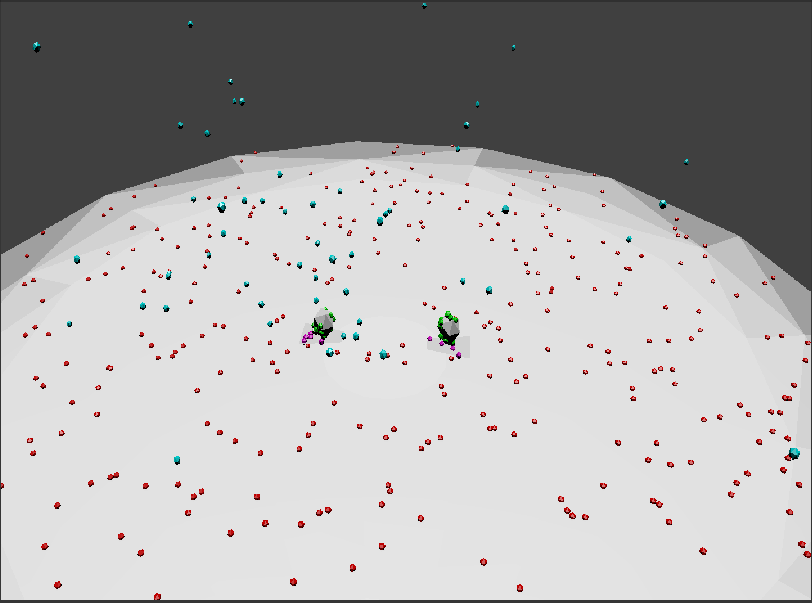
\includegraphics[scale = 0.4]{fig1.png} % requires the graphicx package
   \caption{State of the synapse prior to vesicle release}
   \label{fig1}
\end{figure}
\begin{figure}[H]
   \centering
   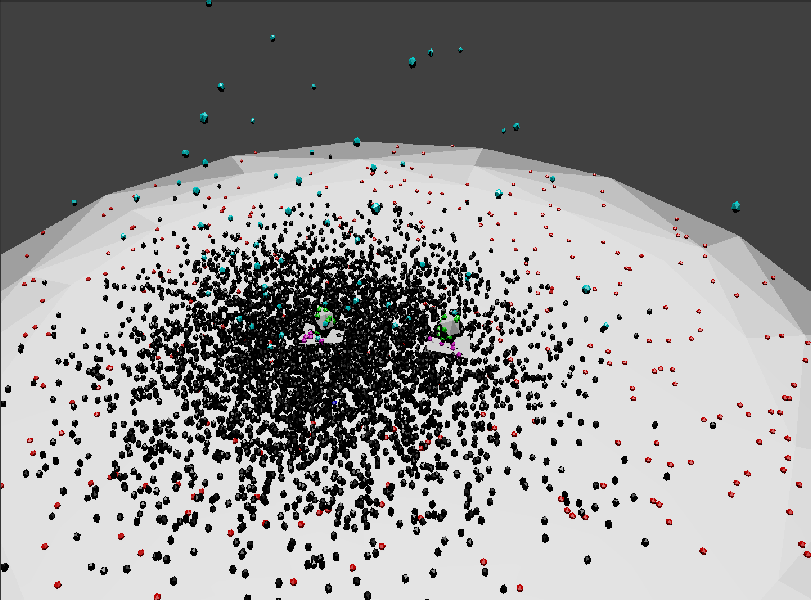
\includegraphics[scale = 0.4]{fig2.png} % requires the graphicx package
   \caption{State of the synapse immediately after vesicle release}
   \label{fig2}
\end{figure}

\begin{figure}[H]
   \centering
   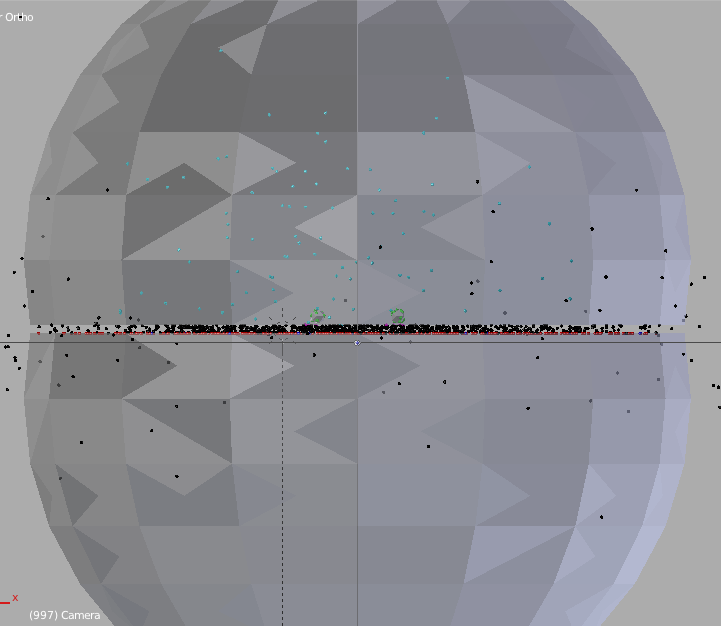
\includegraphics[scale = 0.4]{side_view.png} % requires the graphicx package
   \caption{Side view of the synapse after vesicle release}
   \label{fig3}
\end{figure}

\section{Conclusion}
An implementation of a realistic model of a nerve terminal was produced to demonstrate a method to visualse and model calcium buffering at neocortical nerve terminals. A working model of a spine head and bouton as well as the vesicle release mechanisms within was produced using CellBlender, MCell, Blender and Python. This paper was able to extend the methodology provided in \cite{Czech:MethodsMolBiol:2009} by introducing a method to visualise both the presynaptic and postsynaptic parts of the model simultaneously.

Relevant parameters were obtained from the literature to set up the model in a realistic fashion. Appropriate parameterisation can produce models which are sufficiently realistic to be useful in answering scientific questions. The model can be easily extended to answer a different question - this is merely a matter of introducing the appropriate reactions, molecules, and quantities.

There are many possible extensions to the project. For instance, the model as constructed does not contain much detail in modelling the postsynaptic receptors and their layout on the postsynaptic density. A model with an increased number of vesicles could also be considered, as this would allow for the simulation of the vesicle filling and recycling dynamics.

\section{Acknowledgements}
I would like to thank Jacob Czech of the Pittsburgh Supercomputing Centre for his direct assistance in resolving some technical questions regarding the CellBlender add-on, as well as Markus Dittrich of the same institution for directing the authors queries to Mr. Czech. I would also like to thank \cite{Rollehagen::2015} for allowing the use of their morphology data on L5 synaptic connections. Their paper is currently in preparation and is due to be published later this year. Finally, I would like to thank Christian Stricker for his invaluable help and time in supervising and assisting in the writing of this report.

\bibliography{report_doc}{}
\bibliographystyle{cell}

\end{document}
